% Preámbulo
\documentclass[letterpaper]{article}
\usepackage[utf8]{inputenc}
\usepackage[spanish]{babel}
\decimalpoint

\usepackage{enumitem}
\usepackage{titling}
\usepackage{setspace}

% Símbolos
	\usepackage{amsmath}
	\usepackage{amssymb}
	\usepackage{amsthm}
	\usepackage{amsfonts}
	\usepackage{mathtools}
	\usepackage{bbm}
	\usepackage[thinc]{esdiff}
	\allowdisplaybreaks

% Márgenes
	\usepackage
	[
		margin = 1.2in
	]
	{geometry}
	\onehalfspacing

% Imágenes
	\usepackage{float}
	\usepackage{graphicx}
	\graphicspath{{imagenes/}}
	\usepackage{subcaption}

% Ambientes
	\usepackage{amsthm}

	\theoremstyle{definition}
	\newtheorem{ejercicio}{Ejercicio}

	\newtheoremstyle{lemathm}{4pt}{0pt}{\itshape}{0pt}{\bfseries}{ --}{ }{\thmname{#1}\thmnumber{ #2}\thmnote{ (#3)}}
	\theoremstyle{lemathm}
	\newtheorem{lema}{Lema}

	\newtheoremstyle{lemathm}{4pt}{0pt}{\itshape}{0pt}{\bfseries}{ --}{ }{\thmname{#1}\thmnumber{ #2}\thmnote{ (#3)}}
	\theoremstyle{lemathm}
	\newtheorem{sol}{Solución}
	
	\newtheoremstyle{lemathm}{4pt}{0pt}{\itshape}{0pt}{\bfseries}{ --}{ }{\thmname{#1}\thmnumber{ #2}\thmnote{ (#3)}}
	\theoremstyle{lemathm}
	\newtheorem{theo}{Teorema}

	\newtheoremstyle{lemademthm}{0pt}{10pt}{\itshape}{ }{\mdseries}{ --}{ }{\thmname{#1}\thmnumber{ #2}\thmnote{ (#3)}}
	\theoremstyle{lemademthm}
	\newtheorem*{lemadem}{Demostración}

% Macros
	\newcommand{\sumi}[2]{\sum_{i=#1}^{#2}}
	\newcommand{\dint}[2]{\displaystyle\int_{#1}^{#2}}
	\newcommand{\inte}[2]{\int_{#1}^{#2}}
	\newcommand{\dlim}{\displaystyle\lim}
	\newcommand{\limxinf}{\lim_{x\to\infty}}
	\newcommand{\limninf}{\lim_{n\to\infty}}
	\newcommand{\dlimninf}{\displaystyle\lim_{n\to\infty}}
	\newcommand{\limh}{\lim_{h\to0}}
	\newcommand{\ddx}{\dfrac{d}{dx}}
	\newcommand{\txty}{\text{ y }}
	\newcommand{\txto}{\text{ o }}
	\newcommand{\Txty}{\quad\text{y}\quad}
	\newcommand{\Txto}{\quad\text{o}\quad}
	\newcommand{\si}{\text{si}\quad}

	\newcommand{\etiqueta}{\stepcounter{equation}\tag{\theequation}}
	\newcommand{\tq}{:}
	\renewcommand{\o}{\circ}
	\newcommand*{\QES}{\hfill\ensuremath{\blacksquare}}
	\newcommand*{\qes}{\hfill\ensuremath{\square}}
	\newcommand*{\QESHERE}{\tag*{$\blacksquare$}}
	\newcommand*{\qeshere}{\tag*{$\square$}}
	\newcommand*{\QED}{\hfill\ensuremath{\blacksquare}}
	\newcommand*{\QEDHERE}{\tag*{$\blacksquare$}}
	\newcommand*{\qel}{\hfill\ensuremath{\boxdot}}
	\newcommand*{\qelhere}{\tag*{$\boxdot$}}
	\renewcommand*{\qedhere}{\tag*{$\square$}}

	\newcommand{\suc}[1]{\left(#1_n\right)_{n\in\N}}
	\newcommand{\en}[2]{\binom{#1}{#2}}
	\newcommand{\upsum}[2]{U(#1,#2)}
	\newcommand{\lowsum}[2]{L(#1,#2)}
	\newcommand{\abs}[1]{\left| #1 \right| }
	\newcommand{\bars}[1]{\left \| #1 \right \| }
	\newcommand{\pars}[1]{\left( #1 \right) }
	\newcommand{\bracs}[1]{\left[ #1 \right] }
	\newcommand{\inprod}[1]{\left\langle #1 \right\rangle }
    \newcommand{\norm}[1]{\left\lVert#1\right\rVert}
	\newcommand{\floor}[1]{\left \lfloor #1 \right\rfloor }
	\newcommand{\ceil}[1]{\left \lceil #1 \right\rceil }
	\newcommand{\angles}[1]{\left \langle #1 \right\rangle }
	\newcommand{\set}[1]{\left \{ #1 \right\} }
	\newcommand{\norma}[2]{\left\| #1 \right\|_{#2} }


	\newcommand{\NN}{\mathbb{N}}
	\newcommand{\QQ}{\mathbb{Q}}
	\newcommand{\RR}{\mathbb{R}}
	\newcommand{\ZZ}{\mathbb{Z}}
	\newcommand{\PP}{\mathbb{P}}
    \newcommand{\EE}{\mathbb{E}}
	\newcommand{\1}{\mathbbm{1}}
	\newcommand{\eps}{\varepsilon}
	\newcommand{\ttF}{\mathtt{F}}
	\newcommand{\bfF}{\mathbf{F}}

	\newcommand{\To}{\longrightarrow}
	\newcommand{\mTo}{\longmapsto}
	\newcommand{\ssi}{\Longleftrightarrow}
	\newcommand{\sii}{\Leftrightarrow}
	\newcommand{\then}{\Rightarrow}

	\newcommand{\pTFC}{{\itshape 1er TFC\/}}
	\newcommand{\sTFC}{{\itshape 2do TFC\/}}


% Datos
    \title{Métodos Estadísticos \\ Tarea 3}
    \author{Rubén Pérez Palacios Lic. Computación Matemática\\Profesor: Dr. Rogelio Ramos Quiroga}
    \date{\today}

% DOCUMENTO
\begin{document}
	\maketitle
	
	Considere inferencia Bayesiana sobre el modelo Exponencial.

	\begin{enumerate}
		\item Muestre que la apriori Gamma es conjugada de la distribución Exponencial.
		
		\begin{proof}

			La función de densidad de la distribución Exponencial con parámetro $\lambda$

			\[f(x) = \lambda e^{-\lambda x},\]

			de donde obtenemos 

			\[L\pars{\lambda; x} = \lambda^n e^{-\lambda \sum_{i=1}^{n} x_i}.\]

			La función de densidad de la distribución Gamma con parámetros $\alpha, \theta$ es

			\[\pi\pars{\lambda} = f\pars{\lambda} = \frac{\lambda^{\alpha-1}e^{-\frac{\lambda}{\theta}}}{\Gamma\pars{\alpha}\theta^{\alpha}},\]

			por lo que

			\[\pi\pars{\lambda|x} = \pi(\lambda) L\pars{\lambda; x} \propto \lambda^{\alpha-1}e^{-\frac{\lambda}{\theta}} \lambda^n e^{-\lambda \sum_{i=1}^{n} x_i} = \lambda^{\alpha+n-1}e^{-\lambda\frac{1+\theta\sum_{i=1}^n x_i}{\theta}},\]

			por lo tanto la posterior es $Gamma$ con parametros $\alpha+n, \frac{\theta}{1+\theta\sum_{i=1}^n x_i}$. Concluimos que la apriori Gamma es conjugada de la distribución Exponencial.
		\end{proof}

		\newpage

		\item Suponga que el tiempo de espera en una cola es modelado con la distribución Exponencial$\pars{\lambda}$. Suponga además que, para una muestra aleatoria de $20$ clientes se observó un tiempo medio de espera de $5.1$ minutos. Considere distribuciones previas Gama de dos tipos:
		\begin{enumerate}
			\item Con media $0.5$ y desviación estandar $1$.
			\item Con media $10$ y desviación estandar $20$.
		\end{enumerate}
		Grafique las dos distribuciones posteriores y compárelas.

		\begin{sol}
			Notemos que

			\[\sum_{i=1}^n x_i = 102, \quad n = 20, \quad \alpha\theta = \mu, \quad \alpha\theta^2 = \sigma^2,\]

			por lo que cuando $\mu = 0.5, \sigma = 1$ obtenemos

			\[\pi\pars{\lambda|x} = \frac{102.5^{20.25}\lambda^{19.5}e^{-102.5\lambda}}{\Gamma\pars{20.25}},\]

			y cuando $\mu = 0.5, \sigma = 1$ obtenemos

			\[\pi\pars{\lambda|x} = \frac{102.025^{20.25}\lambda^{19.25}e^{-102.025\lambda}}{\Gamma\pars{20.25}}.\]

			Cuyas gráficas son:

			\begin{figure}[H]
				\centering
				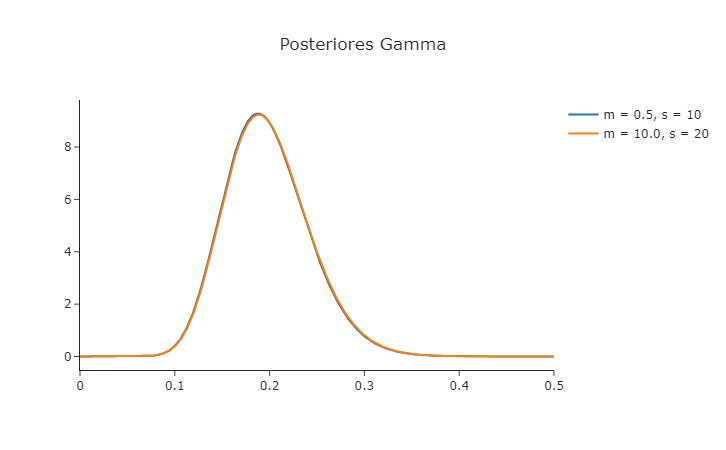
\includegraphics[scale = 0.5]{"../Images/Posteriores.png"}
			\end{figure}

			Las gráficas son muy parecidas.

		\end{sol}
		\item Calcule las dos medias posteriores y compárelas. Explique las diferencias.
		
		\begin{sol}
			Como

			\[\quad \alpha\theta = \mu,\]

			entonces cuando $\mu = 0.5, \sigma = 1$ obtenemos

			\[\mu_{p} = 0.1975,\]

			y cuando $\mu = 10, \sigma = 20$ obtenemos

			\[\mu_{p} = 0.1984.\]

			Ambas medias posteriores son muy parecidas, pero como el parametro de escala es mayor en el segunda es ligeramente más grande su media posterior

		\end{sol}
	\end{enumerate}
\end{document}

